% rm ProjetRecherche.bib ; latex ProjetRecherche.tex ; bibtex ProjetRecherche ; latex ProjetRecherche.tex ; latex ProjetRecherche.tex ; dvips -o projet.ps ProjetRecherche.dvi ; ps2pdf projet.ps

\documentclass[a4paper,12pt]{article}

\usepackage[]{natbib}  

\usepackage{fullpage}

\usepackage{calc}
\usepackage[usenames,dvipsnames]{color}

\usepackage[latin1]{inputenc} 
\usepackage[T1]{fontenc}    
\usepackage{textcomp}
\usepackage{rotating}

\usepackage[frenchb,english]{babel} 
\usepackage{amssymb,amsmath} 
\usepackage{float}
\usepackage{url}                
\usepackage{amstext}
\usepackage{tipa}
%\usepackage{palatino}
\usepackage{fancyvrb}
\DefineVerbatimEnvironment{code}{Verbatim}{fontsize=\small}
\newcommand{\D}{\mathrm{d}}  

\graphicspath{{ManualFig/}}


\begin{document}

\begin{center}
\section*{\Huge{Quick User Guide for \texttt{GYOTO}}}

\vspace{0.5cm}

\Large{Updated}
\today

\vspace{4cm}

\begin{figure}[htbp]
\centering
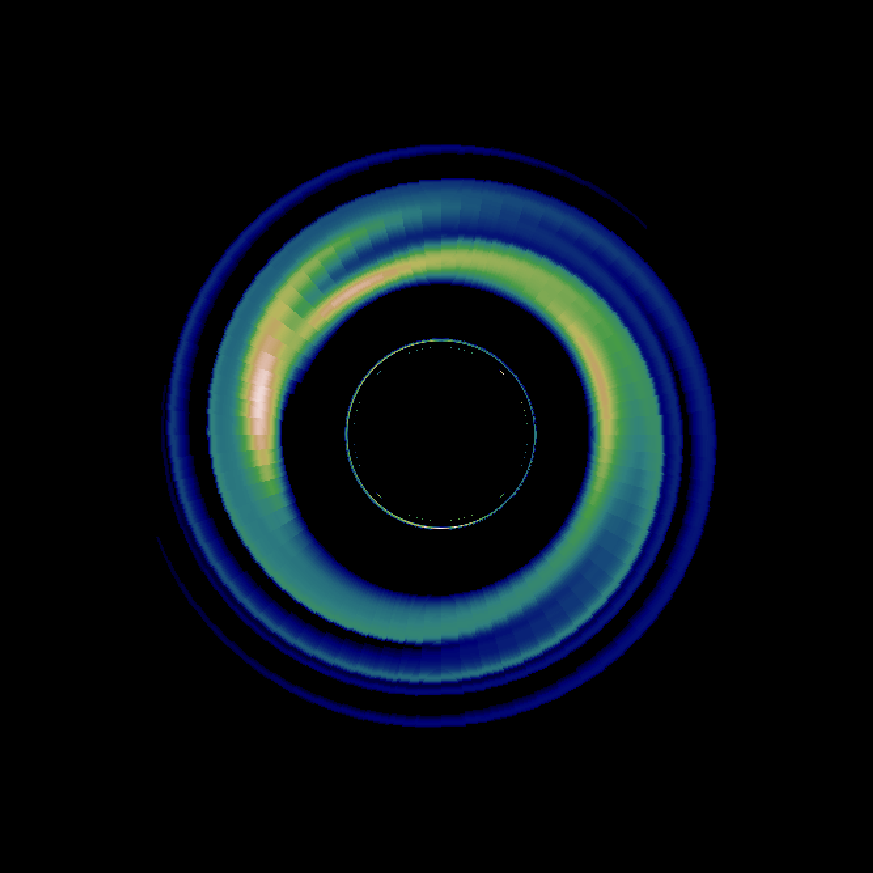
\includegraphics[width=10cm,height=10cm]{RWI_t1822_nu18.pdf}
%\caption{}
%\label{fig:hotspot}
\end{figure}

\end{center}



\newpage

\section*{Introduction - Scope of this Guide}

This Guide aims at giving a general presentation of the \textit{General relativitY Orbit Tracer of Observatoire de Paris}, \texttt{GYOTO} (pronounced \textipa{[dZIoto]}, as for the Italian trecento painter Giotto di Bondone). This text is not a lecture on ray-tracing techniques and is only devoted to presenting the code so that it can be quickly handled by any user. Readers interested in the physics behind \texttt{GYOTO} are referred to~\citet[][and references therein]{vincent11a,vincent12a}. The aim of this Guide is also to present the code in sufficient details so that people interested to develop their own version of \texttt{GYOTO} can do it easily.

\texttt{GYOTO} is an open source C++ code with a Yorick plug-in that computes null and timelike geodesics in the Kerr metric as well as in any metric computed within the framework of the 3+1 formalism of general relativity. This code allows to compute mainly images and spectra of astrophysical sources emitting electromagnetic radiation in the vicinity of compact objects (e.g. accretion disks or nearby stars). 

As \texttt{GYOTO} is continually evolving, this guide will (hopefully) be regularly updated to present the new functionalities added to the code.

The reader is strongly encouraged to give feedback on this Manual, report typos, ask questions or suggest improvements by sending an email to \url{frederic.vincent@obspm.fr}

\tableofcontents



\newpage

\section{Installing \texttt{GYOTO}}
\label{install}

\texttt{GYOTO} is freely available at the URL \url{http://gyoto.obspm.fr/}. This URL hosts the online manual of \texttt{GYOTO}, with installation instructions and brief descriptions of the code architecture.

\texttt{GYOTO} is version-controlled with the \texttt{git} software that you should install on your machine.
Before uploading the code, be sure that the \texttt{xerces-c3} (or \texttt{xercesc3} depending on the
architecture) and \texttt{cfitsio} libraries are installed on your system: \texttt{GYOTO} won't compile without these.
It is also better (but not required) to install the \texttt{udunits2} library. Once this is done, just type on a command line
\begin{code}
git clone git://github.com/gyoto/Gyoto.git
\end{code}  
which will create a \texttt{Gyoto} repository. It contains directories \texttt{bin}, \texttt{lib}, \texttt{include}, \texttt{doc}, \texttt{yorick}
containing respectively the core code and executable, the \texttt{.C} source files, the \texttt{.h} headers, the documentation
and \texttt{Yorick} plug-in related code. 

In the \texttt{Gyoto} repository, use the standard 
\begin{code}
./configure; make; sudo make install 
\end{code}
commands
to build the code.

In case of problems, have a look at the \texttt{INSTALL} file that gives important complementary informations on how to install \texttt{GYOTO}.

\section{A first demonstration}
\label{demo}

A \texttt{GYOTO} computation relies on two kinds of files: an \texttt{XML} file containing the inputs and a \texttt{FITS} file containing the outputs.

\subsection{XML input file}

You can find examples of \texttt{XML} input files in \texttt{doc/examples/}. Let us consider the computation of the image of a standard Page-Thorne accretion disk in Boyer-Lindquist coordinates, described in \texttt{example-page-thorne-disk-BL.xml}. 

\begin{sloppypar} %to allow proper newline for long words (in texttt)
If you are not familiar with \texttt{XML} language, just remember that an \texttt{XML} file is made of several fields beginning with the \texttt{<Field Name>} and ending with \texttt{</Field Name>}. One field can have sub-fields, defined with the same symbols. For instance in \texttt{example-page-thorne-disk-BL.xml}, there is one global field, \texttt{Scenery}, describing the scenery that will be ray-traced, with a few sub-fields: \texttt{Metric} describing the metric used for the computation, here the Kerr metric in Boyer-Lindquist coordinates; \texttt{Screen} describing the observer's screen properties; finally \texttt{Astrobj} describing the astrophysical object that will be ray-traced, here a Page-Thorne accretion disk.
All the parameters in this input file can be changed to specify a new scenery. 

Let us present in details the \texttt{example-page-thorne-disk-BL.xml} file:

\begin{code}
<?xml version="1.0" encoding="UTF-8" standalone="no"?>
<Scenery>
\end{code}

The following lines specify the metric: it is the Kerr metric, expressed in Boyer-Lindquist coordinates, with spin 0 (so the Schwarzschild metric here!):

\begin{code}
  <Metric kind = "KerrBL">
    <Spin>
      0.
    </Spin>
  </Metric>
\end{code}

The metric is now defined, let us describe the observer's screen.
The \texttt{Position} field gives the screen's 4-position 
in Boyer-Lindquist coordinates $(t,r,\theta,\varphi)$, 
angles in radians, time and radius in geometrical units  
(i.e. units with $c$ and $G$ put to 1). The \texttt{Time} field
gives the time of observation. The \texttt{FieldOfView} is given in radians.
The screen's \texttt{Resolution} is the number of screen pixels in each
direction.

\begin{code}
  <Screen>
    <Position>
      1000.
       100.
       1.22
       0.
    </Position>
    <Time unit="geometrical_time">
       1000.   
    </Time>
    <FieldOfView>
       0.314159265358979323846264338327950288419716
     </FieldOfView>
     <Resolution> 
       32   
     </Resolution>
  </Screen>
\end{code}

The screen is now defined. The following line describes the target object that will be ray-traced:

\begin{code}
   <Astrobj kind = "PageThorneDisk"/>
\end{code}

Here the target object is very simple and requires no specifications.
The \texttt{Scenery} is now fully defined and the field can be closed

\begin{code}
  </Scenery>
\end{code}

This is the end of the \texttt{XML} input file!

\end{sloppypar}

\subsection{Calling \texttt{GYOTO}}

Once the \texttt{XML} input file is ready, the call to \texttt{GYOTO} is done according to the following line:

\begin{code}
> gyoto input.xml \!output.fits
\end{code}

where \texttt{input.xml} is the above mentioned \texttt{XML} file and \texttt{output.fits} is the name of the \texttt{FITS} that will contain the result of the computation.
The \texttt{!} before the \texttt{.fits} file allows to overwrite a pre-existing file. If you remove it, an error will occur if the \texttt{.fits} file already exists. 

The line above asks \texttt{GYOTO} to integrate a null geodesic from each pixel of the screen backward in time towards the astrophysical object. You can ask \texttt{GYOTO} to compute only a fraction of the screen's pixels by running:

\begin{code}
> gyoto ----imin=IMIN ----imax=IMAX ----jmin=JMIN ----jmax=JMAX input.xml \!output.fits
\end{code}

where \texttt{IMIN}, \texttt{IMAX}, \texttt{JMIN}, \texttt{JMAX} are the extremal indices of the pixels that will be computed. For instance, to compute only the geodesic that hits the central pixel of a $32 \times 32$ screen, type:
\begin{code}
> gyoto ----imin=16 ----imax=16 ----jmin=16 ----jmax=16 input.xml \!output.fits
\end{code}

\subsection{FITS output file}

Once the computation is performed, the \texttt{output.fits} file is created. You can visualize it by using the \texttt{ds9} software (\url{http://hea-www.harvard.edu/RD/ds9/site/Home.html}) and simply running:

\begin{code}
> ds9 ouput.fits
\end{code}

For instance, if you use the \texttt{example-page-thorne-disk-BL.xml} as is, you will obtain Fig.~\ref{fig:demo}.

\begin{figure}[htbp]
\centering
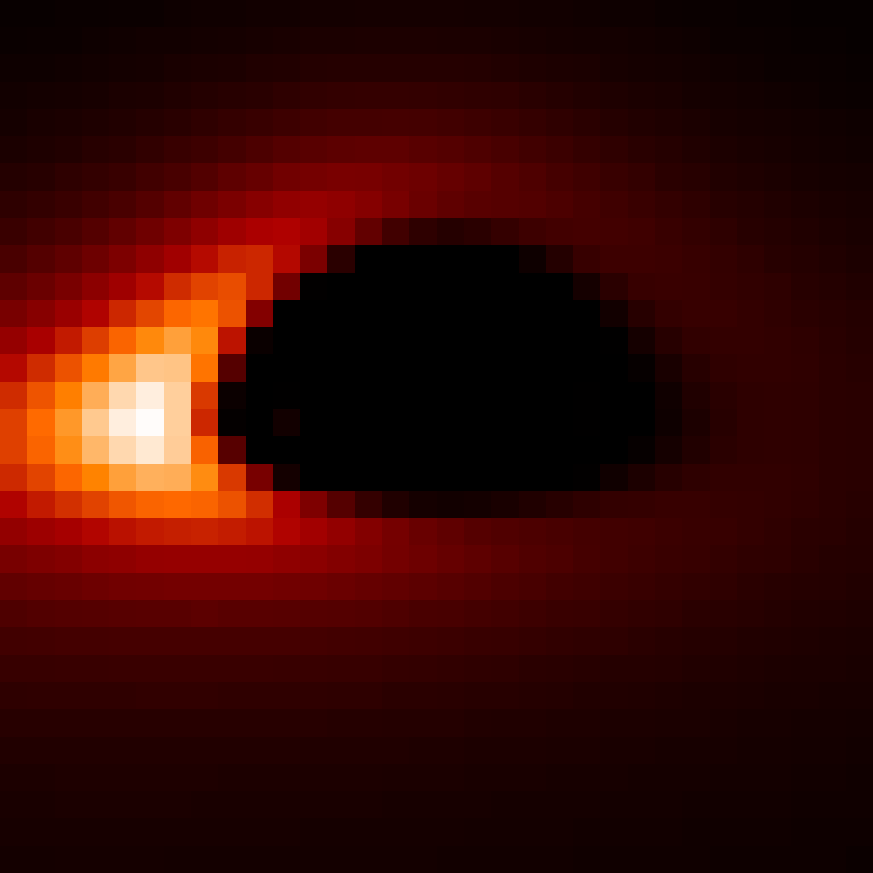
\includegraphics[width=8cm,height=8cm]{DemoPageThorne.pdf}
\caption{Image of a Page-Thorne thin accretion disk around a Schwarzschild black hole, with a $32\times 32$ pixels screen.}
\label{fig:demo}
\end{figure}



\section{\texttt{GYOTO} architecture}
\label{archi}

\subsection{\texttt{GYOTO} base classes}

\texttt{GYOTO} is basically organized around 8 base classes (see Fig.~\ref{fig:hierarch}):

\begin{itemize}
\item The \texttt{Metric} class: it describes the metric of the spacetime (Kerr in Boyer-Lindquist coordinates, Kerr in Kerr-Schild coordinates, metric of a relativistic rotating star in 3+1 formalism...).
\item The \texttt{Astrobj} class: it describes the astrophysical target object that must ray-traced (e.g. a thin accretion disk, a thick 3D disk, a star...).
\item The \texttt{Spectrum} class: it describes the emitted spectrum of the \texttt{Astrobj}.
\item The \texttt{Worldline} class: it gives the evolving coordinates of a timelike or null geodesic. The \texttt{Star} class is a sub-class of \texttt{Worldline} as for the time being a star in \texttt{GYOTO} is only described by the timelike geodesic of its center, with a given fixed radius.
\item The \texttt{WorldlineIntegState} class: it describes the integration of the \texttt{Worldline} in the given \texttt{Metric}.
\item The \texttt{Screen} class: it describes the observer's screen, its resolution, its position in spacetime, its field of view.
\item The \texttt{Scenery} class: it describes the ray-tracing scene. It is made of a \texttt{Metric}, a \texttt{Screen}, an \texttt{Astrobj} and the quantities that must be computed (an image, a spectrum...).
\item The \texttt{Factory} class: it allows to translate the \texttt{XML} input file into C++ objects.
\end{itemize}

Fig.~\ref{fig:hierarch} presents the main \texttt{GYOTO} classes and their hierarchy.

\begin{figure}[htbp]
\centering
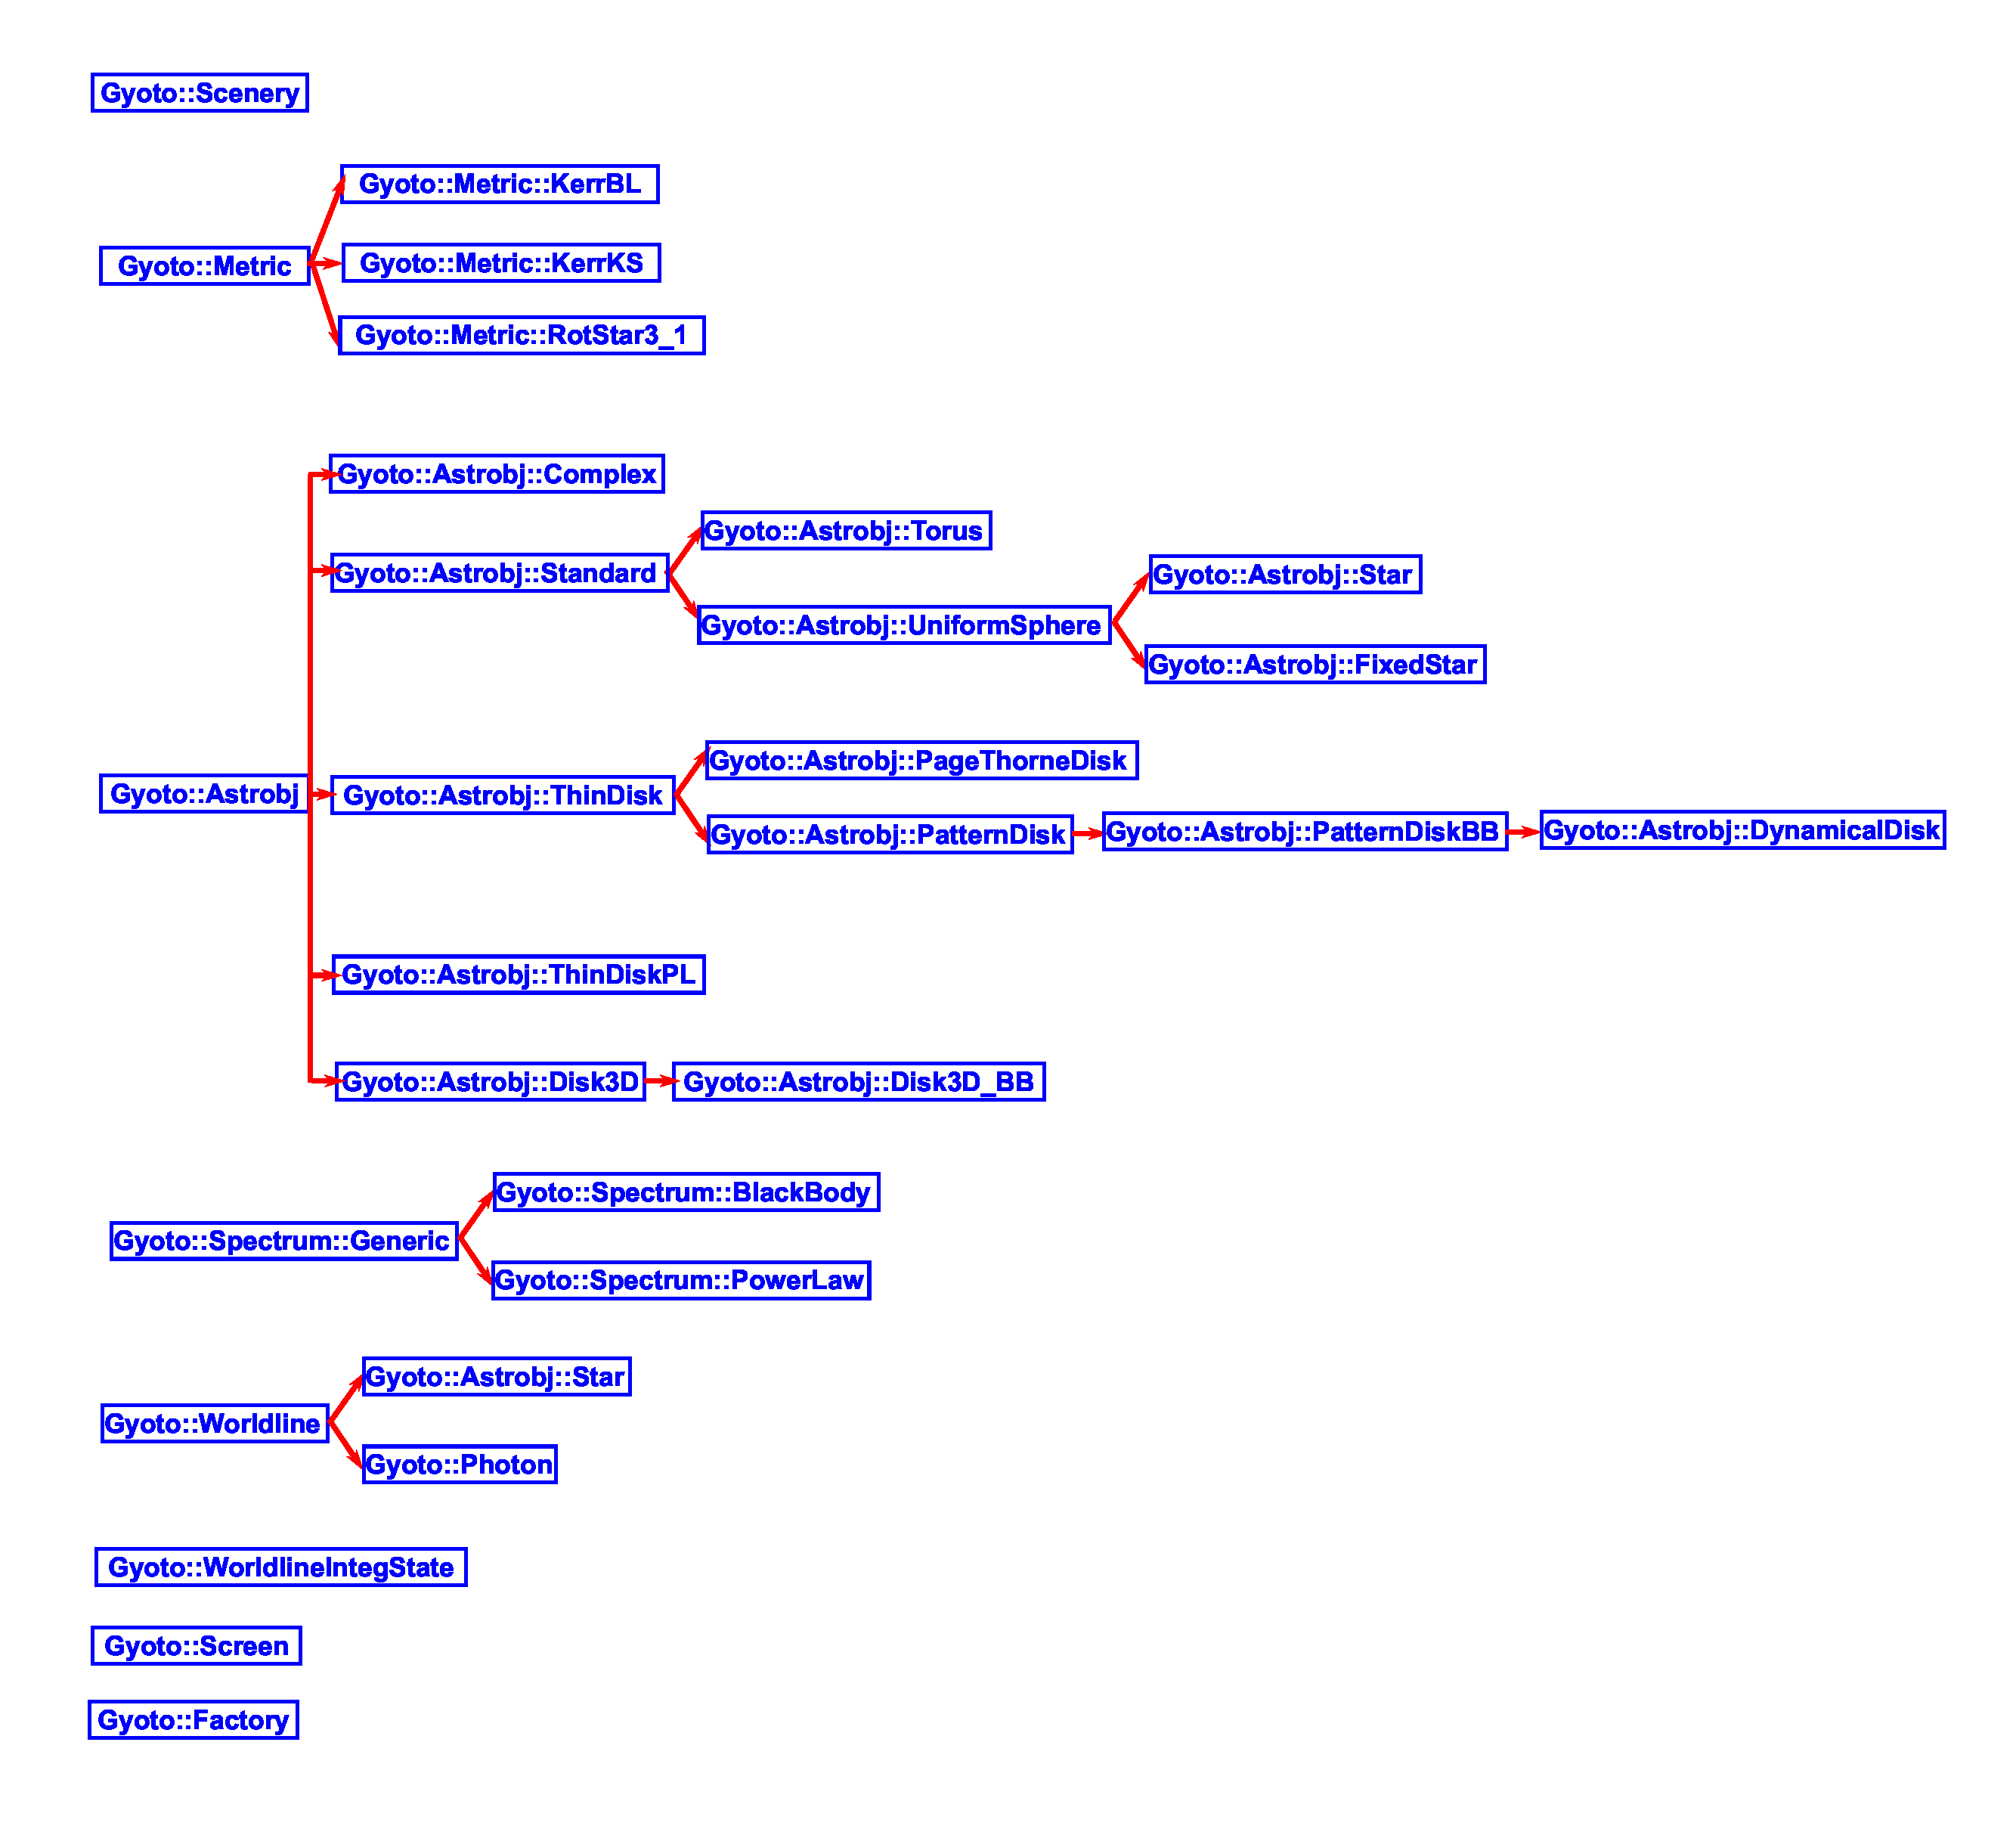
\includegraphics[width=18cm,height=20cm]{ClassHierarch.pdf}
\caption{Hierarchy of \texttt{GYOTO} C++ main classes.}
\label{fig:hierarch}
\end{figure}

\subsection{A typical \texttt{GYOTO} computation}

\begin{sloppypar} %to allow proper newline for long words (in texttt)
Let us now describe the main interactions of these various classes during the computation of one given photon, ray-traced in the Kerr metric in Boyer-Lindquist coordinates towards, for instance, a \texttt{PageThorneDisk}, i.e. a geometrically thin optically thick disk following \citet{page74}.

All directories used in the following are located in \texttt{GYOTO} home directory.

\texttt{GYOTO} \texttt{main} program is located in \texttt{bin/gyoto.C}. This program first interprets the command line given by the user. It creates a new \texttt{Factory} object, initialized by means of the \texttt{XML} input file, that will itself create (see \texttt{lib/Factory.C}) the \texttt{Scenery}, \texttt{Screen} and \texttt{Astrobj} objects. The output quantities the user is interested in (image, spectrum...) will be stored during the computation in the \texttt{data} object, of type \texttt{Astrobj::Properties}. The \texttt{Scenery} object is then used to perform the ray-tracing, by calling its \texttt{rayTrace} function. All the functions that begin with \texttt{fits\_} allow to store the final output quantities in \texttt{FITS} format.

The function \texttt{Scenery::rayTrace} calls \texttt{Photon::hit} that forms the core of \texttt{GYOTO}: \texttt{Photon::hit} integrates the null geodesic from the observer's screen backward in time until the target object is reached (there are other stop conditions of course, see \texttt{lib/Photon.C}). \texttt{Photon::hit} is basically made of a loop that calls the function \texttt{WorldlineIntegState::nextStep} until a stop condition is reached.  \texttt{WorldlineIntegState::nextStep} itself calls the correct adaptive fourth order Runge-Kutta integrator (RK4) , depending on the metric used. Here, the metric being \texttt{KerrBL}, the RK4 used is \texttt{KerrBL::myrk4\_adaptive}. 

Moreover, the \texttt{Photon::hit} also calls the \texttt{Astrobj::Impact} function that asks the \texttt{Astrobj} whether the integrated photon has reached it or not. When the photon has reached the target, this \texttt{Astrobj::Impact} function calls the \texttt{Astrobj::processHitQuantities} function that updates the \texttt{data} depending on the user's specifications. 
\end{sloppypar}

\section{Computing an image or a spectrum in the Kerr metric with \texttt{GYOTO}}
\label{kerr}

\subsection{The \texttt{Screen}}

The observer's \texttt{Screen} is made of $N\times N$ pixels, and has a field of view of $f$ radians. The field of view is defined as the maximum angle between the normal to the screen and the most tangential incoming geodesic. 

Keep in mind that the screen is point-like, the different pixels are all at the same position (the one and only screen position defined in the \texttt{XML} file), but the various pixels define various angles on the observer's sky.  For instance, if $f=\pi / 2$ (which gives a view of the complete half space in front of the screen), the geodesic that hits the screen on the central pixel $(i=N/2,j=N/2)$ comes from the direction normal to the screen whereas the geodesic that hits the screen on the $(i=N,j=N/2)$ pixel comes from a direction tangential to the screen.

Each pixel of the screen thus covers a small solid angle on the observer's sky. This elementary solid angle is equal to the solid angle subtended by a cone of opening angle $f$ divided by the number of pixels: $\delta\Omega_{\mathrm{pixel}} = 2\,\pi\,(1-\cos f) / N^{2}$ (assuming the field of view is small enough).

\subsection{Computing an image}

The quantity that is carried along the geodesics computed by \texttt{GYOTO} in most cases is the specific intensity $I_{\nu}$ ($\mathrm{erg\,cm^{-2}\,s^{-1}\,ster^{-1}\,Hz^{-1}}$).

An image is then defined as a map of specific intensity: each pixel of the screen contains one value of $I_{\nu}$, that can then be plotted. It is important to keep in mind that such an "image" is not physically equivalent to a real image that would be obtained with a telescope: a real image is a map of specific fluxes values, and a specific flux is the sum of the specific intensity on some solid angle.

An example of image computation has already been given in Section~\ref{demo}.


\subsection{Computing a spectrum}



To compute a spectrum, the \texttt{Screen} field of the \texttt{XML} file should contain information about the observed frequency range. For a real telescope, this means adding a spectrometer. The additional command in the \texttt{XML} file is thus:

\begin{code}
<Spectrometer kind="freqlog" nsamples="20">5. 25.</Spectrometer>
\end{code}

This line means that that $20$ values of observed frequencies will be considered, evenly spaced logarithmically, between $10^{5}$ and $10^{25}$ Hz. It is possible to choose frequencies linearly evenly spaced by using \texttt{freq} instead of \texttt{freqlog}. It is also possible to use wavelengths instead of frequencies, see \texttt{GyotoScreen.h} for more information.

Moreover, the \texttt{XML} file should explicitly state that the quantity of interest is no longer a simple image, but a spectrum. This is allowed by the following command, that should be added for instance before the end of \texttt{Scenery} field:

\begin{code}
<Quantities>Spectrum</Quantities>
\end{code}
When this command is used, the output \texttt{FITS} file will contain a cube of images, each image corresponding to one observed frequency.

Computing the spectrum is now straightforward. Remembering that the flux is linked to the intensity by:

\begin{equation}
\D F_{\nu_{\mathrm{obs}}} = I_{\nu_{\mathrm{obs}}}\,\cos\theta\,\D \Omega,
\end{equation}
where $\Omega$ is the solid angle under which the emitting element is seen, and $\theta$ is the angle between the normal to the observer's screen and the direction 
of incidence, the flux is given by:

\begin{equation}
\label{deffluxGyoto}
F_{\nu_{\mathrm{obs}}} = \sum_{\mathrm{pixels}} I_{\nu_{\mathrm{obs}},\mathrm{pixel}}\,\cos(\theta_{\mathrm{pixel}})\,\delta\Omega_{\mathrm{pixel}} ,
\end{equation}
where $I_{\nu_{\mathrm{obs}},\mathrm{pixel}}$ is the specific intensity reaching the given pixel, $\theta_{\mathrm{pixel}}$ is the angle between the normal to the screen and the direction of incidence corresponding to this pixel and $\delta\Omega_{\mathrm{pixel}}$ is the element of solid angle introduced above. 

This quantity $F_{\nu_{\mathrm{obs}}}$ can thus be very simply computed from the cube of specific intensities computed by \texttt{GYOTO}. Examples of spectra computed by \texttt{GYOTO} can be found in, e.g.,~\citet{straub12}.


\section{\texttt{GYOTO} in numerical metrics}
\label{3+1}

A specificity of \texttt{GYOTO} is its ability to ray-trace in non-Kerr metrics, numerically computed in the framework of the 3+1 formalism of general relativity~\citep{gourgoulhon12}, e.g. by means of the open source LORENE library developed by the Numerical Relativity group at Observatoire de Paris/LUTH\footnote{\url{http://www.lorene.obspm.fr/}}. 

\begin{sloppypar}
For the time being, only a simple example of numerical metric is implemented in the public version of \texttt{GYOTO}: the metric of a relativistic rotating star. The file \texttt{doc/examples/example-movingstar-rotstar3\_1.xml} allows to ray-trace a basic \texttt{GYOTO} moving \texttt{Star} in this metric. The file \texttt{resu.d} specified in the \texttt{XML} file is the output of a LORENE computation for the metric of a rotating relativistic star by the LORENE/nrotstar code.
\end{sloppypar}

The basic functions developed in \texttt{lib/RotStar3\_1.C} are similar to their Kerr counterparts, but here the metric is expressed in terms of the 3+1 quantities (lapse, shift, 3-metric, extrinsic curvature). The equation of geodesics expressed in the 3+1 formalism is given in~\citet{vincent12a} and implemented in \texttt{lib/RotStar3\_1.C}. However, it is possible to choose in the \texttt{XML} file whether the integration will be performed by using this 3+1 equation of geodesics, or by using the most general 4D equation of geodesics~\citep[see][for a comparison of the two methods]{vincent11a}.

\section{\texttt{GYOTO} Yorick plug-in}
\label{yorick}

[In construction...]
 
\section{Adding a new astrophysical target object in \texttt{GYOTO}}
\label{newastrobj}

[In construction...]

\bibliographystyle{aa}  % A&A bibliography style file (aa.bst)
\bibliography{GyotoManual}


\end{document}

% Local IspellDict: francais